\chapter{\ifproject%
\ifenglish Project Structure and Methodology\else โครงสร้างและขั้นตอนการทำงาน\fi
\else%
\ifenglish Project Structure\else โครงสร้างของโครงงาน\fi
\fi
}

ในบทนี้จะกล่าวถึงโครงสร้างของระบบในภาพรวม ขั้นตอนการทํางานของระบบ อุปกรณ์ หน้าที่ของอุปกรณ์ กลวิธีการต่าง ๆ และซอฟต์แวร์ที่ใช้ในระบบ โดยขั้นตอนการทํางานจะมี 9 ขั้นตอน
โดยจะแบ่งระบบออกเป็นเป็น 2 ส่วนใหญ่ ๆ คือส่วนของมอดูลกล้อง และเซิร์ฟเวอร์

\makeatletter

% \renewcommand\section{\@startsection {section}{1}{\z@}%
%                                    {13.5ex \@plus -1ex \@minus -.2ex}%
%                                    {2.3ex \@plus.2ex}%
%                                    {\normalfont\large\bfseries}}

\makeatother
%\vspace{2ex}
% \titleformat{\section}{\normalfont\bfseries}{\thesection}{1em}{}
% \titlespacing*{\section}{0pt}{10ex}{0pt}

\section{ภาพรวมโครงสร้างและการทำงานของระบบ}


\begin{figure}[ht!]
  \begin{center}
    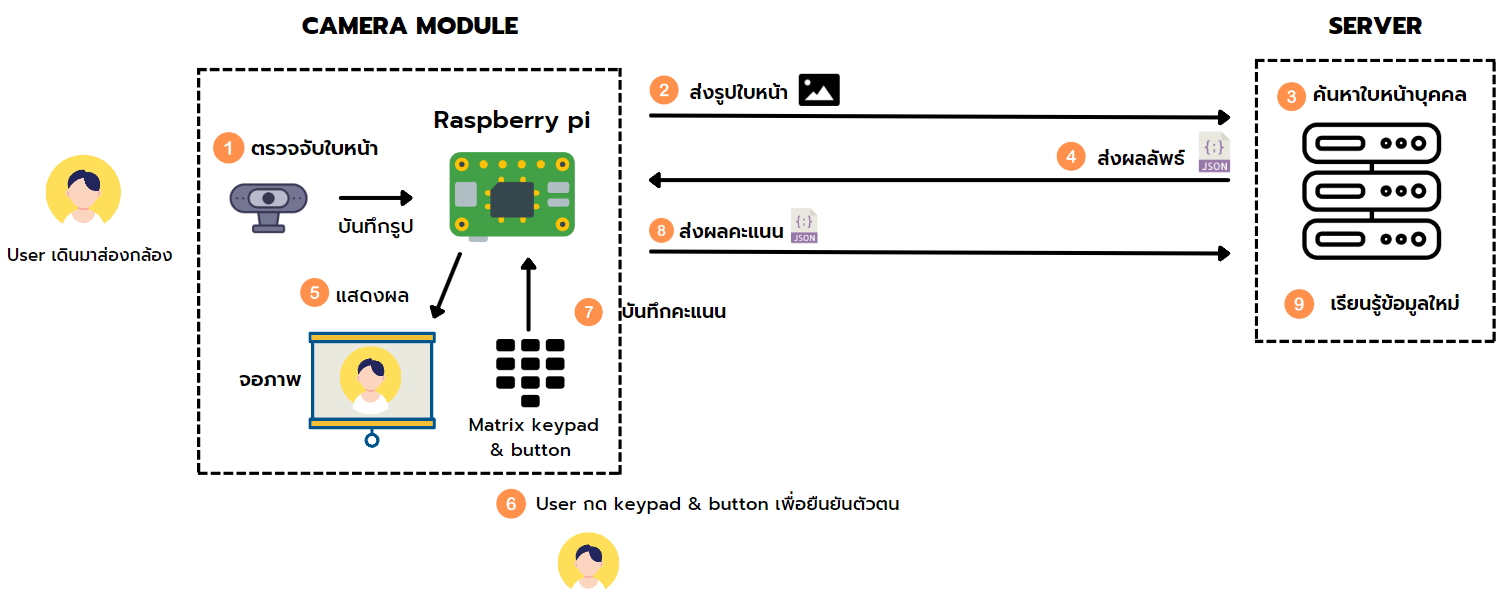
\includegraphics[scale=.5]{pic/overview.png}
  \caption[ภาพรวมของระบบ]{ภาพรวมของระบบ}
  \end{center}
  \label{fig:overview}
\end{figure}

\textbf{ขั้นตอนการทำงานของระบบมีดังนี้}
\begin{enumerate}
  \item เมื่อผู้ใช้งานเดินมาส่องกล้องแล้วมอดูลกล้องจะทำการตรวจจับใบหน้า
  \item บันทึกและส่งรูปภาพใบหน้าไปยังเซิร์ฟเวอร์ในรูปแบบแฟ้มข้อมูลภาพกราฟิกส์สีเครือข่ายใช้ได้หลายระบบ (Portable Network Graphics: PNG) 
        ผ่านโพรโทคอลเอชทีทีพี (HTTP)
  \item เชิร์ฟเวอร์รับรูปภาพแล้วบันทึกรูปภาพเพื่อนำไประบุตัวตนของรูปภาพกับแบบจำลอง (model)
  \item เชิร์ฟเวอร์ส่งผลลัพธ์ของการระบุตัวตนกลับไปยังมอดูลกล้อง (Camera module) ในรูปแบบแฟ้มข้อมูลเจซัน (JSON)
  \item แสดงผลการระบุตัวตนทางหน้าจอ
  \item ผู้ใช้งานกดแผงแป้นพิเศษ (Matrix keypad) หรือ ปุ่มกดเพื่อยืนยันตัวตน
  \item บันทึกผลการกดยืนยันตัวตน
  \item ส่งผลการยืนยันตัวตนไปยังเซิร์ฟเวอร์
  \item นำรูปภาพใบหน้าที่มีการยืนยันตัวตนไปจัดเก็นในฐานข้อมูลของบุคคนนั้น ๆ แล้วจึงทำการเรียนรู้รูปภาพใบหน้าที่ได้รับเข้ามาใหม่ในเวลากลางคืน หรือช่วงเวลาที่มีผู้ใช้งานน้อย
\end{enumerate}

\subsection{มอดูลกล้อง (Camera Module)}

\begin{figure}[ht!]
  \begin{center}
    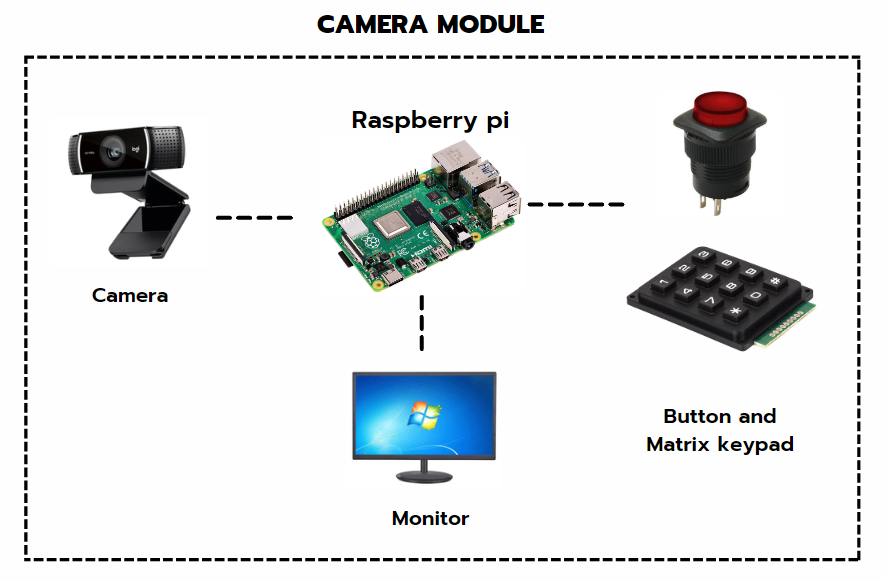
\includegraphics[scale=.45]{pic/camera_module.png}
    \caption[ส่วนประกอบต่าง ๆ ที่ใช้ในมอดูลกล้อง (Camera Module)]{ส่วนประกอบต่าง ๆ ที่ใช้ในมอดูลกล้อง (Camera Module)}
    \label{fig:camera}
  \end{center}
\end{figure}

\textbf{อุปกรณ์ที่ใช่ในมอดูลกล้องสำหรับการตรวจจับใบหน้ามีดังนี้}
\begin{enumerate}
  \item Raspberry Pi 4 Model B : แพลตฟอร์มที่ใช้ในการค้นหาใบหน้าบุคคล ซึ่งคุณสมบัติที่จำเป็นได้แก่ 
  มีขนาดเล็ก สามารถส่งข้อมูลผ่านเครื่องข่ายไร้สายไวไฟ (WI-FI) หรือผ่านเครือข่ายที่ใช้สาย (LAN) สามารถอ่านข้อมูลภาพจากกล้องถ่ายภาพ 
  และส่งรูปภาพไปยังเซิร์ฟเวอร์และรอรับผลลัพธ์ และส่งผลลัพธ์จากปุ่มกลับไปยังเซิร์ฟเวอร์
  \item Camera : กล้องเว็บแคมที่มีใช้มาการส่งภาพใบหน้าไปยัง Raspberry Pi
  \item Monitor : หน้าจอแสดงผลที่ใช้ในการแสดงผลลัพธ์ของการระบุตันตน
  \item Button และ Matrix keypad : ใช้ในการรับการให้คะแนนการแสดงผลลัพธ์และแก้ไขความถูกผิดของการแสดงผลลัพธ์
\end{enumerate}

\subsection{การส่งข้อมูลไปยังเซิร์ฟเวอร์}
การส่งรูปภาพจากมอดูลกล้องไปยังเซิร์ฟเวอร์นั้นในมอดูลกล้องใช้คำสั่ง ภาษาไพธอน (Python) ในการใช้สั่งคำส่งของระบบ (System)
คือเคิร์ล  (Client for URLs: cURL) ในการส่งรูปภาพผ่าน HTTP ไปยังเซิร์ฟเวอร์ที่เป็น (RESTful Web Services: RWS)
ผ่านเลขที่อยู่ไอพี (IP Address) ของเซิร์ฟเวอร์ โดย RWS นั้นใช้ Flask Framework 
ในการสร้างเนื่องจาก Flask Framework นั้นใช้ภาษาไพธอน (Python) ในการเขียนทำให้มีความสะดวกในการเรียก OpenCV มาใช้งาน

\subsection{การแสดงผลการระบุตัวตน}
การแสดงผลทางหน้าจอที่เชื่อมต่อกับ Raspberry Pi โดยรับข้อมูลมาจากเซิร์ฟเวอร์ในรูปแบบ JSON ที่มีข้อมูลผลลัพธ์การระบุตัวตน แล้วนำข้อมูลมาวิเคราะห์
ผลลัพธ์การระบุตัวตนจะต้องมีความน่าจะเป็นมากกว่า 80 เปอร์เซ็นต์จะแสดงผลลัพธ์ของบุคคลที่มีความน่าจะเป็นมากที่สุด แต่ถ้ามีความใกล้เคียงน้อยกว่า 80 เปอร์เซ็นต์ก็จะแสดงผลว่า ``ไม่รู้จัก"
และเมื่อผลลัพธ์มีความน่าจะเป็นของการระบุตัวตนระหว่าง 60 ถึง 80 เปอร์เซ็นต์ก็จะให้ผู้ใช้งานป้อนรหัสยืนยันตัวตน

\begin{figure}[!ht]
  \begin{center}
    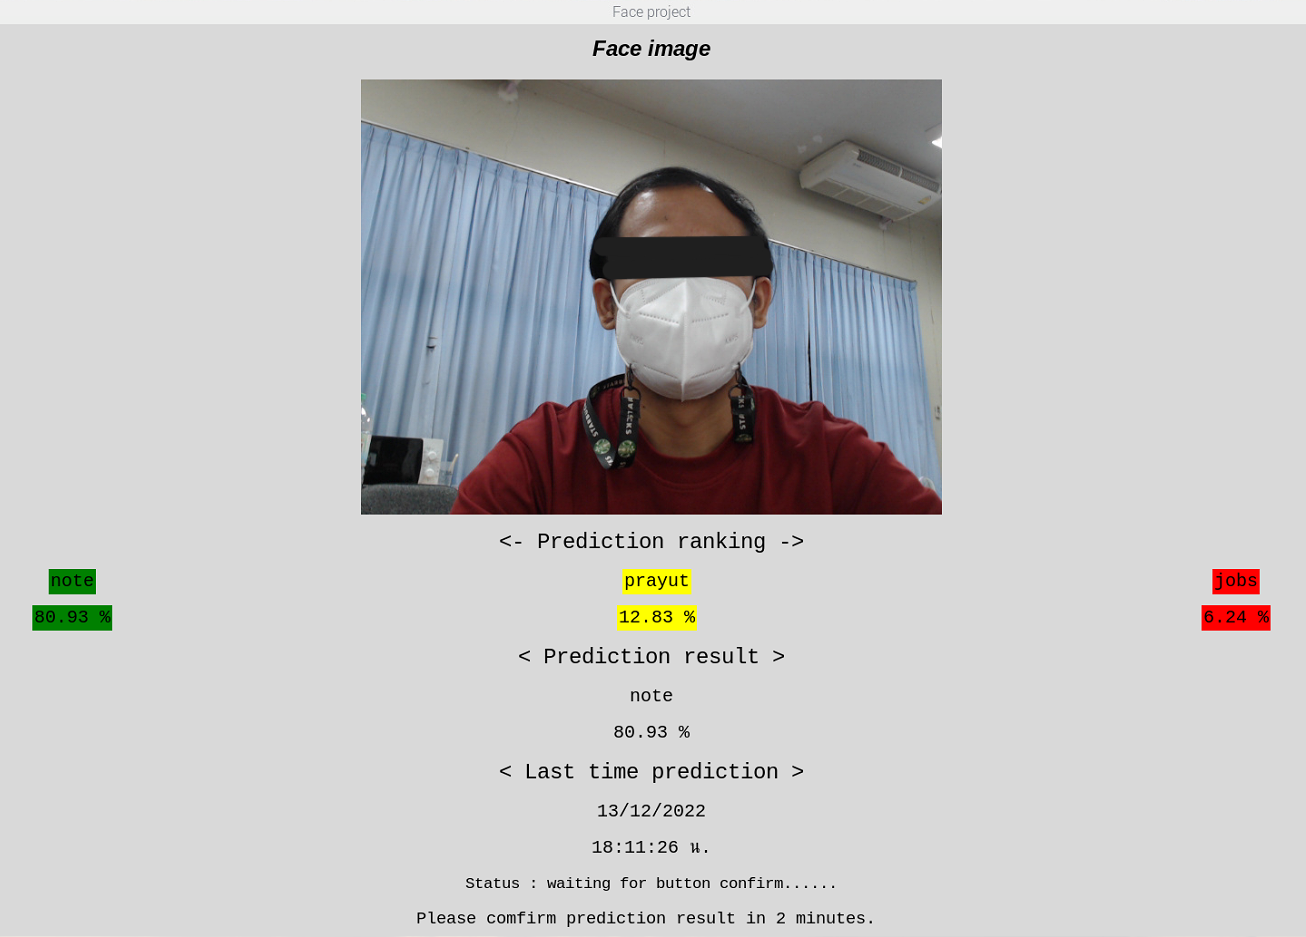
\includegraphics[scale=.45]{pic/result_page_blind.png}
  \caption[แสดงผลลัพธ์การระบุตัวตน]{แสดงผลลัพธ์การระบุตัวตน}
  \end{center}
  \label{fig:predict_result}
\end{figure}


\section{เซิร์ฟเวอร์ (Server)}
ทำหน้าที่ในการเป็นเว็ปเซอร์วิส (Web service) ในการรับรูปภาพเพื่อนำรูปภาพมาระบุตัวตนโดยใช้ OpenCV
เพื่อบอกว่ารูปภาพใบหน้าที่ได้รับเข้ามามีความใกล้เคียงกับบุคคลในฐานข้อมูล โดยแบบจำลอง (model) ที่ใช้ในการระบุตัวตนนั้นมาจาก OpenFace ที่ได้เรียนรู้รูปภาพใบหน้าจากที่จัดเก็บ (Storage) 
จนได้แบบจำลอง (model) ไปใช้งานในการระบุตัวตน และเมื่อ OpenCV บอกผลลัพธ์ได้แล้วจึงทำการส่งการตอบสนอง (Response) 
กลับไปยังมอดูลกล้อง แล้วทำการรอรับข้อมูลการยืนยันตัวตนเพื่อนำรูปภาพที่ได้รับเข้ามาใหม่นั้นย้ายไปยังตำแหน่งที่จัดเก็บของบุลคลนั้น ๆ ในเวลากลางคืนหรือเสลาที่มีผู้ใช้งานน้อยของทุก 
วัน เซิร์ฟเวอร์จะทำการสั่ง OpenFace เรียนรู้รูปภาพใหม่ และนำแบบจำลอง (model) ใหม่ไปใช้งาน โดยเซิร์ฟเวอร์จะมีความต้องการด้านฮาร์ดแวร์คือต้องมีความจุมากกว่า 1 เทราไบต์  (Terabyte) 
หน่วยความจำขนาด 16 จิกะไบต์ (Gigabyte) ในการประมวลผล

\subsection{การระบุตัวตน}
การระบุตัวตนจะใช้ภาพถ่ายใบหน้าที่ได้รับมาจากมอดูลกล้อง โดยใช้ OpenFace ในการระบุตัวตน และใช้แบบจำลอง (model) ที่มีการเรียนรู้จากรูปภาพที่ได้รับเข้ามาก่อนหน้า 
และนำมาใช้ในการระบุตัวตนของรูปภาพใบหน้าที่ได้รับเข้ามาใหม่ แล้วนำผลลัพธ์การระบุตัวตนส่งข้อมูลไปให้เซิร์ฟเวอร์เพื่อทำการส่งผลลัพธ์การระบุตัวตนกลับไปยังมอดูลกล้อง

\subsection{การจัดเก็บรูปภาพใบหน้า}
จัดเก็บรูปภาพใบหน้าลงในที่เก็บข้อมูลในเครื่อง (Local storage) บนเซิร์ฟเวอร์โดยแบ่งเป็นแฟ้มข้อมูล \\(Folder) 
ในแต่ละแฟ้มก็จะเป็นรายชื่อของบุคคลที่ลงทะเบียนหรือเป็นผู้ที่ใช้งานห้อง 
โดยเมื่อได้รับรหัสการยืนยันตัวตนในกรณีที่ความแม่นยำการระบุตัวตนระหว่าง 60 ถึง 80 เปอร์เซ็นต์จากการระบุตัวตน จะทำการเที่ยบรหัสที่ได้รับเข้ามากับรหัสที่จัดเก็นบนฐานข้อมูล 
เมื่อผลลัพธ์การเทียบมีความถูกต้องจะย้ายรูปภาพไปยังแฟ้มของบุคคลนั้น แต่ถ้าผลลัพธ์การเทียบไม่ถูกต้อง
จะย้ายรูปภาพไปยังแฟ้มของอื่น ๆ เพื่อให้ผู้ดูแลมาทำการเทียบด้วยตัวอง

\begin{figure}[ht]
  \begin{center}
    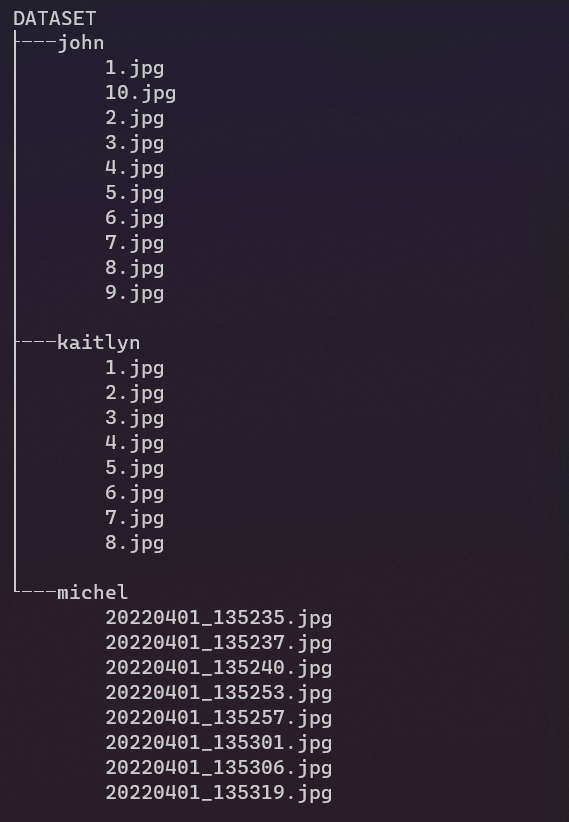
\includegraphics[scale=.5]{pic/dataset.png}
  \caption[แผนภาพแสดงการจัดเก็บรูปภาพใบหน้า]{แผนภาพแสดงการจัดเก็บรูปภาพใบหน้า}
  \end{center}
  \label{fig:folder}
\end{figure}

\subsection{การตรวจสอบรหัสยืนยันตัวตน}
การแสดงผลทางหน้าจอที่เชื่อมต่อกับ Raspberry Pi โดยรับข้อมูลรหัสยืนยันตัวตนจากผู้ใช้งานที่กรอกรหัสยืนยันตัวตนทาง Keypad เป็นเลขจำนวน 6 หลัก
แล้วส่งข้อมูลไปยังเซิร์ฟเวอร์เพื่อทำการตรวจเช็ครหัสกับฐานข้อมูล แล้วจะส่งผลลัพธ์การตรวจเช็คกลับไปยังมอดูลกล้อง
โดยเซิร์ฟเวอร์ส่งข้อมูลในรูปแบบ JSON กลับมาให้ Raspberry Pi แบบการสนอง (Response) เมื่อรับข้อมูลจากเซิร์ฟเวอร์จะนำไปแสดงผลที่หน้าจอ 
\newpage
\begin{figure}[ht]
  \begin{center}
    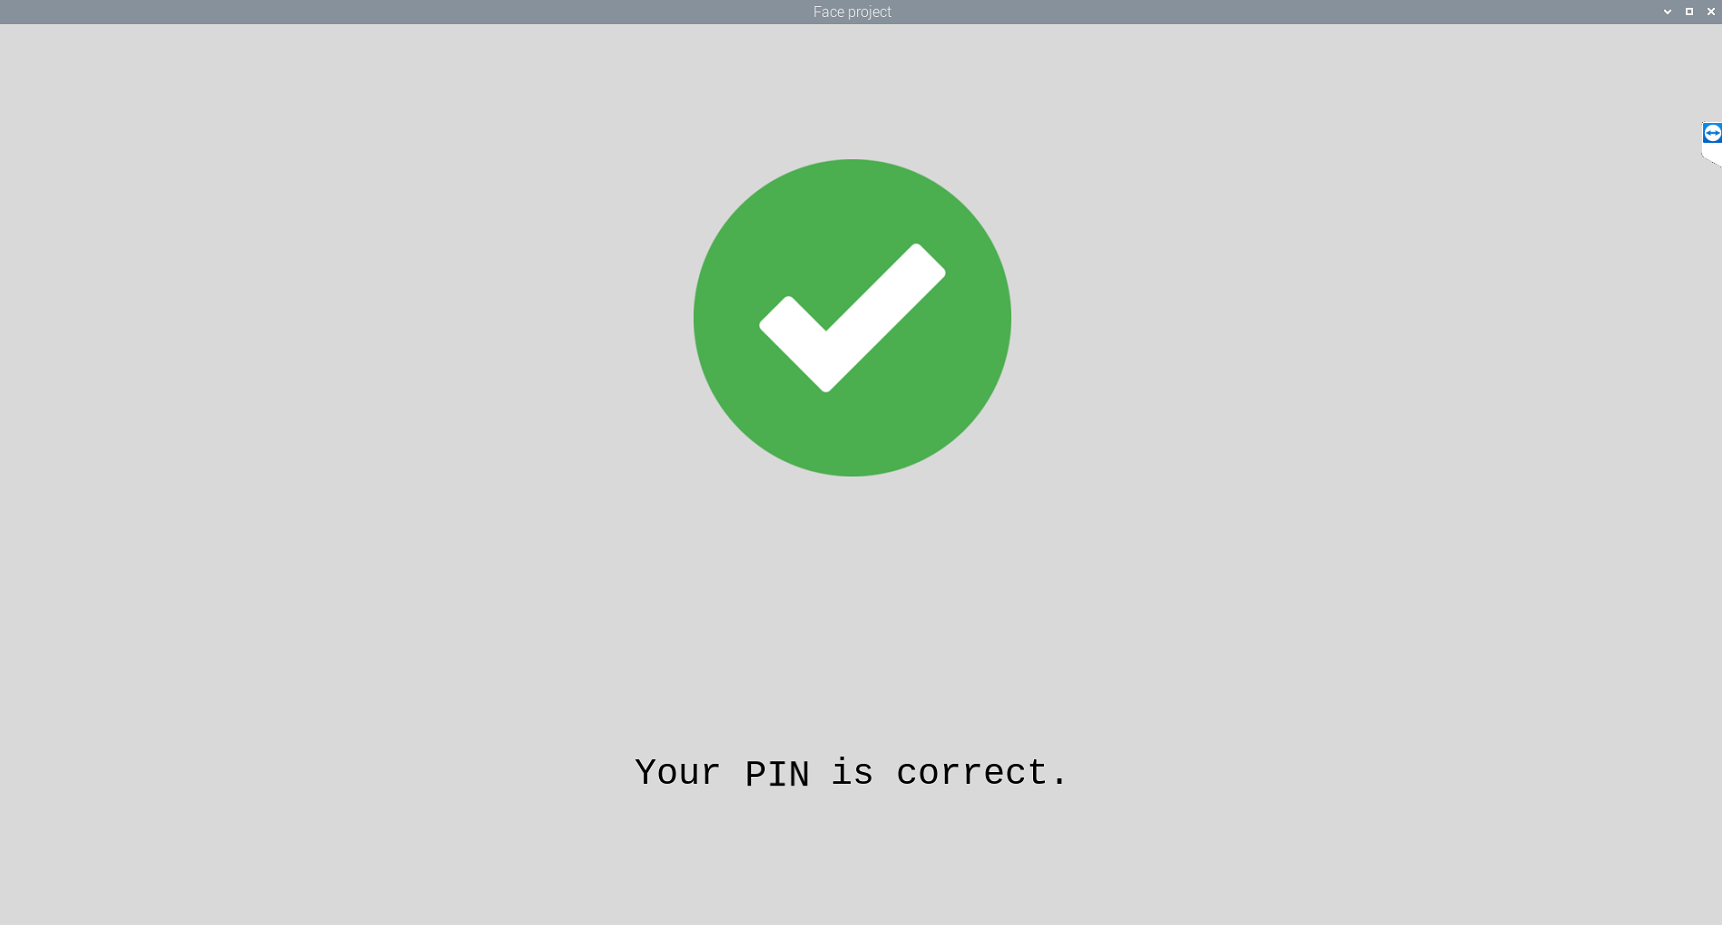
\includegraphics[scale=.3]{pic/pin_correct.png}
  \caption[แสดงผลลัพธ์การกรอกรหัส เมื่อผลลัพธ์ถูกต้อง]{แสดงผลลัพธ์การกรอกรหัส เมื่อผลลัพธ์ถูกต้อง}
  \end{center}
  \label{fig:confirmT}
\end{figure}

\begin{figure}[ht]
  \begin{center}
    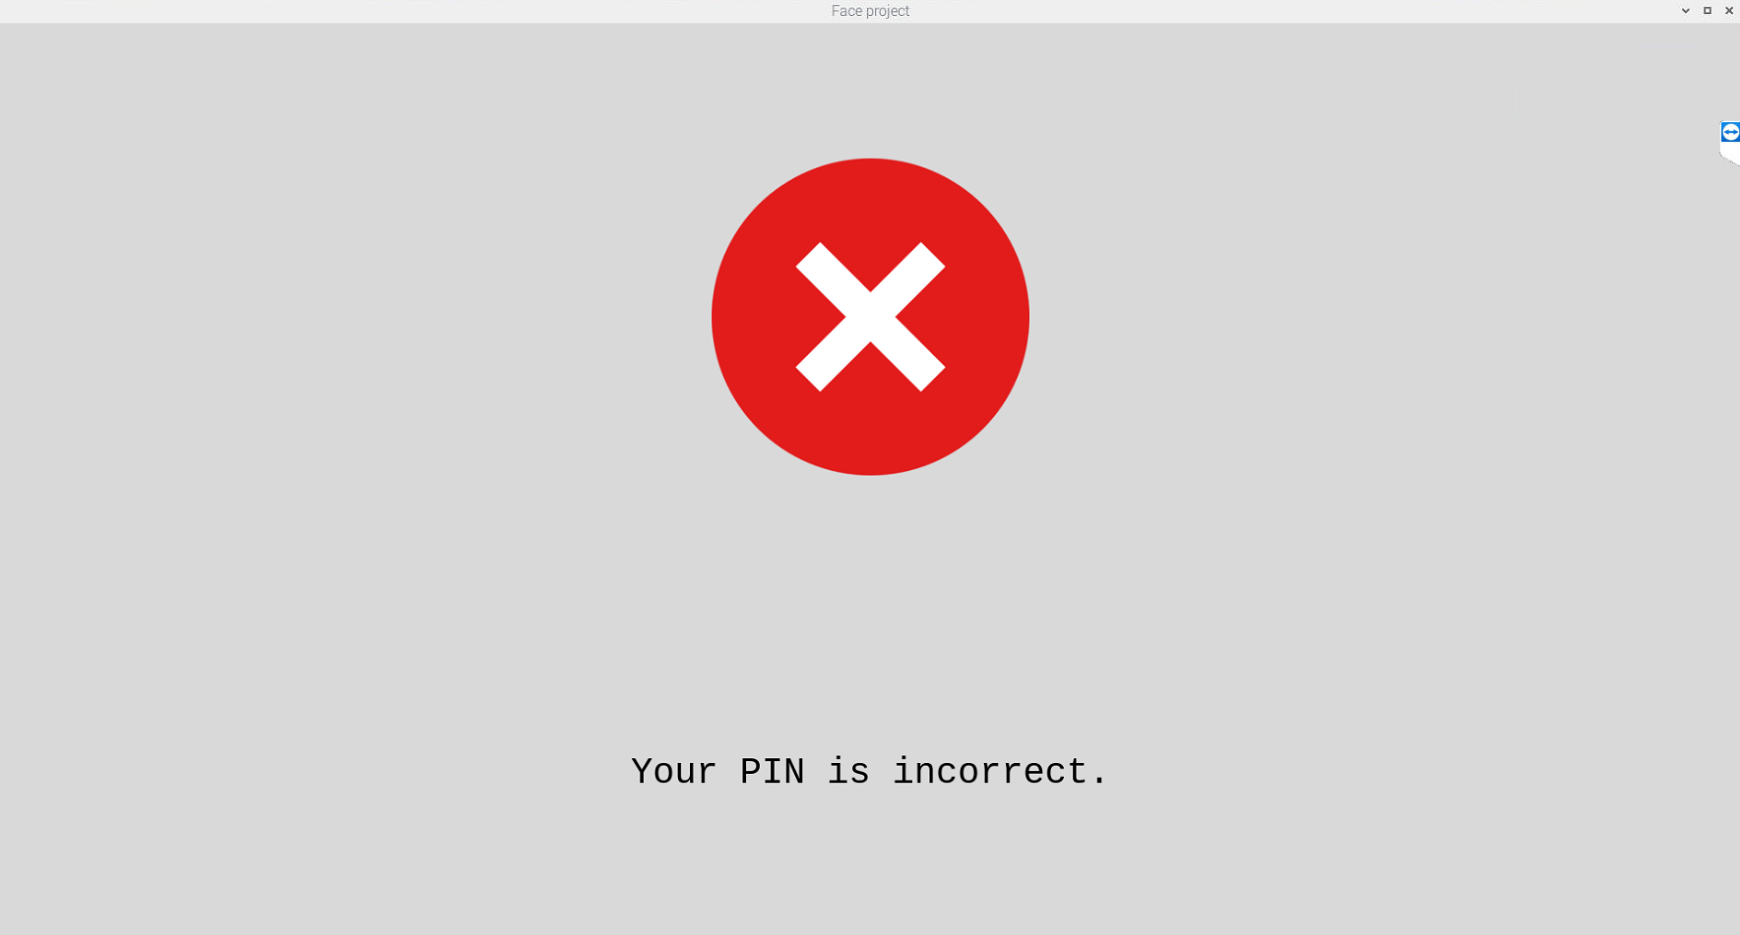
\includegraphics[scale=.3]{pic/pin_incorrect.png}
  \caption[แสดงผลลัพธ์การกรอกรหัส เมื่อผลลัพธ์ไม่ถูกต้อง]{แสดงผลลัพธ์การกรอกรหัส เมื่อผลลัพธ์ไม่ถูกต้อง}
  \end{center}
  \label{fig:confirmF}
\end{figure}

\section{การเรียนรู้รูปภาพ}
ใช้ OpenFace ในการเรียนรู้รูปภาพ โดย OpenFace นั้นใช้ภาษาไพธอน (Python) ในการเขียนโปรแกรมเพื่อเรียนรู้รูปภาพใบหน้า เริ่มจากการนำรูปภาพของบุคคลที่บันทึกไว้ในที่จัดเก็บ (Storage) 
และรายชื่อของบุคคลที่มีรูปภาพใบหน้าในที่จัดเก็บ (Storage) แล้วทำการเรียนรู้ด้วย OpenFace จะได้แบบจำลองการเรียนรู้เพื่อนำไปใช้ในการระบุตัวตนของบุคคล 
โดยขั้นตอนการเรียรรู้จะใช้เวลาขึ้นอยู่กับจำนวนของรูปภาพที่จัดเก็บไว้และใช้ทรัพยากรในการเรียนรู้รูปภาพใบหน้าที่สูงจึงนำ OpenFace ไปทำการเรียนรู้ที่เซิร์ฟเวอร์

% do with it:---it was the black kitten's fault entirely~\cite{aiw}.  For the

